\documentclass[
journal=jctcce,
layout=twocolumn
]{achemso}

\setkeys{acs}{
	abbreviations = false,
	articletitle  = false,
	keywords      = false,
	maxauthors    = 10,
	super         = true
}
% Comment below before submitting
\let\titlefont\undefined
\usepackage[fontsize=11pt]{scrextend}
\usepackage[hidelinks,colorlinks,citecolor=blue]{hyperref}
%\flushbottom
% Comment above before submitting

\usepackage{xr}
\externaldocument{rigid_bodies_supp_info}
\usepackage{booktabs}
\usepackage{threeparttable}
\usepackage{amsmath}
\usepackage{amssymb}
\usepackage[T1]{fontenc}
\usepackage[table]{xcolor}
\definecolor{lightgray}{gray}{0.9}
\usepackage{tikz}
\usetikzlibrary{decorations.text}
\newcommand{\mt}[1]{\boldsymbol{\mathbf{#1}}}   % matrix symbol
\newcommand{\vt}[1]{\boldsymbol{\mathbf{#1}}}   % vector symbol
\newcommand{\tr}[1]{#1^\text{t}}                % transposition
\newcommand{\diff}[2]{\frac{\partial #1}{\partial #2}} % derivative
\newcommand{\sdiff}[2]{\nabla^2_{#2}#1}         % 2nd derivative
\newcommand{\Ham}[1]{{\mathcal H}_\text{#1}}    % Hamiltonian
\newcommand{\Liu}[1]{i\!L_\text{#1}}            % Liouville
\newcommand{\timestep}{h}
\newcommand{\refined}[1]{\widetilde{#1}}

\usepackage{array}
\newcolumntype{L}{>{$}l<{$}}
\newcolumntype{C}{>{$}c<{$}}
\newcolumntype{R}{>{$}r<{$}}
\usepackage{booktabs}    
\usepackage[exponent-product=\times]{siunitx}

\newenvironment{smallarray}[1]                          % small arrays
{\null\,\vcenter\bgroup\scriptsize
	\renewcommand{\arraystretch}{1.5}
	\arraycolsep=.13885em
	\hbox\bgroup$\left[\array{@{}#1@{}}}
{\endarray\right]$\egroup\egroup\,\null}
\listfiles

\author{Ana J. Silveira}
\email{asilveira@plapiqui.edu.ar}
\affiliation{Planta Piloto de Ingenier\'ia Qu\'imica, PLAPIQUI, Universidad Nacional del Sur, Camino La Carrindanga Km 7-CC: 717, Bah\'ia Blanca, Argentina}

\author{Charlles R. A. Abreu}
\email{abreu@eq.ufrj.br}
\affiliation{Chemical Engineering Department, Escola de Qu\'imica, Universidade Federal do Rio de Janeiro, Rio de Janeiro, RJ 21941-909, Brazil}

\title{Refinement of Thermostated Molecular Dynamics via Backward Error Analysis}

\keywords{aaa, bbb, ccc}

\begin{document}

%\begin{tocentry}
%\end{tocentry}

%\begin{abstract}
%\end{abstract}

\section{Introduction}

Molecular dynamics (MD) simulation involves several types of approximations in the quest for mimicking real systems.
Naively, we tend to rank simulation results by their proximity to experimental data and attribute any disagreement to a lack of accuracy of the force field.
However, systematic errors can possibly be hidden in these deviations, being the cause of non-physical behavior.
For instance, it has been shown \cite{Eastwood_2010} that errors due to the discretization of the equations of motion appear to disrupt the equipartition of kinetic energy among molecules of distinct sizes.
A similar artifact occurs for the partition of kinetic energy between translational and rotational degrees of freedom of rigid bodies \cite{Davidchack_2010, Silveira_2017}.
This brings into question the NVT-MD integrator developed by \citeauthor{Kamberaj_2005} \cite{Kamberaj_2005} in which, assuming translational-rotational equipartition, separate chains of Nos\'{e}-Hoover thermostats are coupled to the two classes of degrees of freedom.
In addition, as we will show later on, this method fails to reproduce the specified temperature even for a time-step size $\timestep$ typically employed in MD.
In fact, \citeauthor{Davidchack_2010} \cite{Davidchack_2010} recommends that the use of separate thermostats for translation and rotation should always be avoided.
Nevertheless, issues arise even for freely-moving particles or when translation and rotation are coupled to a single thermostat.
This occurs because Nos\'{e}-Hoover chains (NHC) \cite{Martyna_1992} and other thermostat methods routinely used in MD are based on the relation between temperature and kinetic energy that is a corollary of the equipartition theorem.

For a symplectic integration of Hamiltonian equations of motion, the breakage of equipartition is arguably only apparent \cite{Eastwood_2010}.
The produced trajectory actually follows the dynamics dictated by a \textit{shadow Hamiltonian} \cite{Tuckerman_2010}, which is no longer separable into exclusively momentum- and position-dependent parts and only coincides with the specified Hamiltonian when $\timestep \to 0$.
Therefore, what seems to occur in fact is a failure to identify the quantity that is subject to equipartition in place of the specified kinetic energy.
As \citeauthor{Eastwood_2010} \cite{Eastwood_2010} have shown, Tolman's generalized equipartition theorem \cite{Tolman_1918} holds at least for small steps, when such a \textit{shadow kinetic energy} keeps displaying a quadratic dependency on the momenta.
The authors then employed backward error analysis to successfully eliminate the artifacts mentioned above.
Here, we prove that their findings can be extended to the symplectic integration of rigid-body motion.

It seems then reasonable to argue that a NHC thermostat should regulate the shadow kinetic energy instead of the specified one.
However, the theory underlying the concept of shadow Hamiltonian is only applicable to symplectic integrators, whereas NHC thermostats introduce non-Hamiltonian components to the equations of motion.
In this paper, we devise a novel procedure that partially overcomes this limitation.
It consists in using a splitting-based numerical integrator that entails a Hamiltonian component and carrying out backward error analysis out of this NVE part only.
This allows us to obtain, with minimal computational overhead, a \textit{refined kinetic energy} and a \textit{refined Hamiltonian} as suitable estimators of their shadow counterparts.
By recasting the thermostat equations with this refined kinetic energy, we are able to predict its equipartition and to reproduce a canonical ensemble consistent with the refined Hamiltonian.
Finally, a reweighting procedure provides us with ensemble averages which are, instead, consistent with the specified one. It should be emphasized that this approach is not limited to deterministic thermostats. It would be straightforward to use it, for instance, in conjunction with global stochastic thermostats such as those of \citeauthor{Bussi_2007} \cite{Bussi_2007} and \citeauthor{Leimkuhler_2009} \cite{Leimkuhler_2009}, for instance.

Our new method is particularly appealing for rigid-body MD, primarily because its numerical stability extends up to time steps large enough to yield pronounced discretization errors. Rigid-body MD is relevant not only because some molecules are usually modeled as rigid, such as in the ubiquitous case of water \cite{Jorgensen_1983}, but also because it can provide a coarse-graining strategy for molecules that can be designed as collections of interconnected bodies, such as proteins and nanoparticles \cite{Miller_2002, Knorowski_2012, Patra_2013}.
In fact, the approach of \citeauthor{Kamberaj_2005} \cite{Kamberaj_2005}, which is implemented in software packages such as HOOMD-\textit{blue}\cite{Anderson_2008} and LAMMPS\cite{Plimpton_1995}, has been applied to simulate small molecules \cite{Geiger_2013, Aimoli_2014, Aimoli_2014_2}, as well as membranes \cite{Bucior_2012}, molecular motors \cite{Akimov_2012}, micelles \cite{Yan_2008}, and nanoparticles \cite{Patra_2014}.
The case of rigid water exemplifies this behavior and serves as an excellent testbed for our proposal.
In fact, we were able to correct the discretization errors in numerically computed averages for time-step sizes up to 6 fs, outperforming both the double-chain method by \citeauthor{Kamberaj_2005} \cite{Kamberaj_2005} and a reimplementation of the single-chain method by \citeauthor{Martyna_1996} \cite{Martyna_1996} for rigid bodies.

This paper proceeds as follows.
In Secs.~\ref{sec:nve}-\ref{sec:nvt} we review the rigid-body dynamics in the NVE and NVT ensembles.
This is followed by our developments on backward error analysis, which we employ in Sec.~\ref{sec:refined_method} to derive our new NVT scheme, whose performance we assess in Sec.~\ref{sec:numerical_results}.
Finally, we present some concluding remarks in Sec.~\ref{sec:conclusion}. Appendix \ref{sec:rigid body shadow hamiltonian} contains a detailed derivation of the shadow Hamiltonian approximation.

\section{Methodology}
\label{sec:methodology}

\subsection{Hamiltonian Dynamics with Rigid Bodies: Notation and Symplectic Integration}
\label{sec:nve}

In a previous paper \cite{Silveira_2017}, we took advantage of a particular factorization of the orientation matrix expressed in terms of quaternion components to
1) derive a new exact solution for torque-free rotations and use it as part of a symplectic integrator for rigid bodies and
2) reinterpret the approximate NO-SQUISH method \cite{Miller_2002} and unveil its equivalence to the earlier method by Dullweber and co-workers \cite{Dullweber_1997}.

The Hamiltonian system of ordinary differential equations (ODE) that describes the rigid-body motion is given by \cite{Silveira_2017}
\begin{subequations}
	\label{eq:ODE system for NVE}
	\begin{align}
%
	&\dot{\vt r} =
	%+\diff{\Ham{}}{\vt p} =
	{\mt M}^{-1} {\vt p}, \\
%
	&\dot{\vt p} =
	%-\diff{\Ham{}}{\vt r} = 
	{\vt F}, \\
%
	&\dot{\vt q} =
	%+\diff{\Ham{}}{\vt \pi} =
	\frac{1}{2} \mt B(\vt q) \vt \omega, \text{ and} \label{eq:EDO_q} \\
%
	&\dot{\vt \pi} =
	%-\diff{\Ham{}}{\vt q} =
	\frac{1}{2} \mt B(\vt \pi) \vt \omega + 2 \mt C(\vt q) \vt \tau. \label{eq:EDO_pi}
	\end{align}
\end{subequations}

In these equations, $\vt r$ is the center-of-mass position of the body, $\vt p$ is its linear momentum, $\vt q$ is a unit quaternion that determines its orientation, and $\vt \pi$ is the quaternion-conjugate momentum.
Vectors $\vt F$ and $\vt \tau$ are, respectively, the resultant force and torque exerted on the body, both represented in the space-fixed frame of reference, and $\vt \omega = \frac{1}{2} {\mt I}^{-1} \tr{\mt B}(\vt q) {\vt \pi}$ is the three-dimensional angular velocity in the body-fixed frame.
Matrices $\mt M$ and $\mt I$ are diagonal ones.
The former contains the body mass in all three diagonal entries while the latter contains the three principal moments of inertia.
Finally, the matrix-valued functions $\mt B$ and $\vt C$ are defined as
\begin{equation*}
\label{eq:def_B_and_C}
\mt B(\vt q) = \begin{smallarray}{rrrr}
-q_2 & -q_3 & -q_4 \\
 q_1 & -q_4 &  q_3 \\
 q_4 &  q_1 & -q_2 \\
-q_3 &  q_2 &  q_1
\end{smallarray}
%
\; \text{and} \;
%
\mt C(\vt q) = \begin{smallarray}{rrrr}
-q_2 & -q_3 & -q_4 \\
 q_1 &  q_4 & -q_3 \\
-q_4 &  q_1 &  q_2 \\
 q_3 & -q_2 &  q_1
\end{smallarray}.
\end{equation*}

The factorization which played a central role in Ref.~\citenum{Silveira_2017} is ${\mt A}(\vt q) = \tr{\mt B}(\vt q) {\mt C}(\vt q)$, where ${\mt A}(\vt q)$ is the rotation matrix that connects the body-fixed and space-fixed frames. Eq.~\eqref{eq:ODE system for NVE} preserves the constraints $\tr{\vt q}{\vt q} = 1$ and $\tr{\vt q}{\vt \pi} = 0$, as well as the value of a Hamiltonian
\begin{equation}
\label{eq:Hamiltonian}
\Ham{} = K(\vt p, \vt q, \vt \pi) + U(\vt r,\vt q),
\end{equation}
where $K$ and $U$ are the kinetic and potential energies of the body, respectively.
While $U(\vt r, \vt q)$ is an arbitrary function, the kinetic energy is given by
\begin{equation}
\label{eq:kinetic energy}
K = \frac{1}{2} \tr{\vt p} {\mt M}^{-1} {\vt p} + \frac{1}{8} \tr{\vt \pi} {\mt B}(\vt q) {\mt I}^{-1} \tr{\mt B}(\vt q) {\vt \pi}.
\end{equation}

Eqs.~\eqref{eq:ODE system for NVE} to \eqref{eq:kinetic energy} can also represent a system of $N$ interacting rigid bodies if we consider that vectors $\vt r$, $\vt p$, $\vt q$, and $\vt \pi$ contain the corresponding properties of all bodies piled together.
The size of diagonal matrices $\mt M$ and $\mt I$ also increases to $3N \times 3N$ in this case.
In addition, $\mt B(\vt q)$ and $\mt C(\vt q)$ become block-diagonal matrices with $4N$ rows and $3N$ columns.
Yet, the notation can be made even more general if $\vt r$, $\vt p$, and $\mt M$ are enlarged further so as to accommodate a number of freely moving atoms.

A numerical solution of Eq.~\eqref{eq:ODE system for NVE} is usually represented by a stepwise application of the classical time-evolution propagator \cite{Tuckerman_2010} $e^{\timestep \Liu{\tiny NVE}}$ to the system configuration, where $\timestep$ is the time-step size and $\Liu{\tiny NVE}$ is the Liouville operator associated to $\Ham{}$, which is
\begin{equation}
\label{eq:Lioville operator}
\begin{split}
\Liu{\tiny NVE} &= \tr{\vt p} {\mt M}^{-1} \diff{}{\vt r} + \frac{1}{2} \tr{\vt \omega} \tr{\mt B}(\vt q) \diff{}{\vt q} + \tr{\vt F} \diff{}{\vt p} \\
&+ \left[ \frac{1}{2} \tr{\vt \omega} \tr{\mt B}(\vt \pi) + 2 \tr{\vt \tau} \tr{\mt C}(\vt q) \right] \diff{}{\vt \pi}.
\end{split}
\end{equation}

A symplectic, time-reversible integrator can be devised by splitting the exponential operator according to the Trotter-Suzuki formula \cite{Trotter_1959, Suzuki_1976}
\begin{equation}
\label{eq:splitting NVE}
e^{\timestep \Liu{\tiny NVE}} = e^{\frac{\timestep}{2} \Liu{B}} e^{\timestep \Liu{A}} e^{\frac{\timestep}{2} \Liu{B}} + \mathcal{O}(\timestep^3),
\end{equation}
where $\Liu{A} + \Liu{B} = \Liu{\tiny NVE}$.
In the Verlet-type splitting of Ref.~\citenum{Silveira_2017}, the action of propagator $e^{\frac{\timestep}{2} \Liu{B}}$ is a kick in the linear and quaternion momenta given by ${\vt p} = {\vt p}^\ast + \frac{\timestep}{2} {\vt F}^\ast$ and ${\vt \pi} = {\vt \pi}^\ast + \timestep {\mt C}({\vt q^\ast}) {\vt \tau}^\ast$, respectively, where the asterisk denotes the state of the system immediately before the propagation occurs.
The action of $e^{\timestep \Liu{A}}$ is a simultaneous uniform translation (${\vt r} = {\vt r}^\ast + \timestep {\mt M}^{-1} {\vt p}^\ast$) and torque-free rotation along a full time step.
We have derived \cite{Silveira_2017} an exact solution for torque-free rotations in a form that facilitates computer implementation and allows, differently from other existing solutions \cite{Kosenko_1998, vanZon2007, Celledoni_2008}, a unified treatment of asymmetric, symmetric, and spherical tops.
This solution was used to evaluate the simpler NO-SQUISH method \cite{Miller_2002}.
Despite its approximate treatment of rotations, which are split into several revolutions around the principal axes \cite{Dullweber_1997}, that method proved to be very accurate in liquid-phase simulations \cite{Silveira_2017}.
This justifies its more widespread use.
However, having an unplit solution for rotations at hand is crucial for the feasibility of backward error analysis, as it might become clear in Sec.~\ref{sec:modified_h} and Appendix \ref{sec:rigid body shadow hamiltonian}.

\subsection{NVT Dynamics with a Single Thermostat Chain: Notation and Measure-Preserving Integration}
\label{sec:nvt}

In this work, we couple a single Nos\'{e}-Hoover chain thermostat \cite{Martyna_1992} to both the translational and rotational degrees of freedom of the rigid-body system.
To this end, we consider an extra generalized coordinate $\eta_j$ and its conjugate momentum $p_{\eta_j}$ for each thermostat $j = 1, \cdots, M$.
The flow in the extended phase-space no longer conserves the Hamiltonian $\Ham{}$, but an \textit{extended energy} given by \cite{Martyna_1992}
\begin{equation}
\label{eq:nvt extended energy}
H = K + U + {\textstyle\sum\limits_{j=1}^{M}} \frac{p_{\eta_j}^2}{2Q_j} + L k_\text{\tiny B} T\eta_1 + k_\text{\tiny B} T {\textstyle\sum\limits_{j=2}^{M}} \eta_j,
\end{equation}
where $k_\text{\tiny B}$ is the Boltzmann constant, $T$ is the target temperature, $L$ is a constant to be determined, and each $Q_j$ is an inertial parameter.
As recommended in Ref.~\citenum{Martyna_1992}, we can make $Q_1 = L k_\text{\tiny B} T t_d^2$ and $Q_j = k_\text{\tiny B} T t_d^2$ for $j \geq 2$, where $t_d$ is a characteristic time scale of the thermostat chain.

By employing the method of Sergi and Ferrario \cite{Sergi_2001}, we obtain the equations of motion for the NVT dynamics with a single thermostat chain, which are
\begin{subequations}
	\label{eq:ODE system for NVT}
	\begin{align}
\label{eq:nhc_r}
	&\dot{\vt r} =
	{\mt M}^{-1} {\vt p}, \\
%
\label{eq:nhc_p} 
	&\dot{\vt p} =
	{\vt F} - \alpha_1 {\vt p},\\
%
\label{eq:nhc_q}
	&\dot{\vt q} =
	\frac{1}{2} \mt B(\vt q) \vt \omega, \\
%
\label{eq:nhc_pi}
	&\dot{\vt \pi} =
	\frac{1}{2} \mt B(\vt \pi) \vt \omega + 2 \mt C(\vt q) \vt \tau - \alpha_1 {\vt \pi}, \\
%
\label{eq:nhc_eta}
	&\dot{\eta}_j = \alpha_j, \text{ and} \\
%
\label{eq:nhc_p_eta}
	&{\dot p}_{\eta_j} = G_j - \alpha_{j+1} p_{\eta_j} \qquad \text{for} \quad 1 \leq j \le M.
	\end{align}
\end{subequations}

In these equations, $\alpha_j$ $=$ ${p_{\eta_j}}/{Q_j}$ for $j \le M$ and $\alpha_{M+1} = 0$, while $G_j$ is a generalized force acting on thermostat $j$, defined as
\begin{subequations}
\begin{align}
\label{eq:generalized force NVT}
&G_1 = \tr{\vt p} \diff{K}{\vt p} + \tr{\vt \pi} \diff{K}{\vt \pi} - L k_\text{\tiny B} T \quad \text{and}\\
&G_j = \frac{p_{\eta_{j-1}}^2}{Q_{j-1}} - k_\text{\tiny B} T  \qquad \text{for} \quad j > 1.
\end{align}
\end{subequations}

With $K$ defined as in Eq.~\eqref{eq:kinetic energy}, it turns out that $G_1 = 2K - L k_\text{\tiny B} T$.
If there are no external forces, the vector quantity $e^{\eta_1}\sum_{i=1}^N {\vt p}_i$ and the extended energy $H$ are conserved, while the system's center-of-mass position and the $\eta$ coordinates can be considered as a driven variables \cite{Tuckerman_2001}.
Moreover, $2N$ equations must be eliminated due to the constraints involving $\vt q$ and $\vt \pi$.
In the general case, by taking all these facts into account and applying the analysis of \citeauthor{Tuckerman_2001} \cite{Tuckerman_2001}, we can deduce that the correct canonical distribution is attained if we make $L = 6N$.
In a particular situation in which we set $\sum_{i=1}^N {\vt p}_i = \vt 0$ at the onset of the simulation, we must make $L = 6N - 3$ \cite{Martyna_1994}.

Eq.~\eqref{eq:ODE system for NVT} defines an invariant measure in the extended phase-space \cite{Tuckerman_1999}, and it is possible to devise numerical solvers that preserve such measure \cite{Sergi_2001, Ezra_2004, Ezra_2006}.
We have done it by adapting the integrator introduced by \citeauthor{Martyna_1996} \cite{Martyna_1996} in light of a criterion explained by \citeauthor{Ezra_2006} \cite{Ezra_2006}.
It is worth noting, however, that such adaptation required us to alter the integration of the $\eta$ coordinates only.
Since these are driven variables, with no influence on the dynamics of the system, we can conclude that the practical importance of such alteration is small.

By defining a propagator $e^{\timestep \mathcal{L}_\text{\tiny NVT}}$, where $\mathcal{L}_\text{\tiny NVT}$ is a generalized (i.e. non-Hamiltonian) Liouville operator, the splitting goes as
\begin{equation}
\label{eq:splitting NVT}
e^{\timestep \mathcal{L}_\text{\tiny NVT}} = e^{\frac{\timestep}{2} \mathcal{L}_\text{\tiny NHC}} e^{\timestep \Liu{\tiny NVE}} e^{\frac{\timestep}{2} \mathcal{L}_\text{\tiny NHC}} + \mathcal{O}(\timestep^3),
\end{equation}
where $\Liu{\tiny NVE}$ is the same operator of Sec.~\ref{sec:nve} and $\mathcal{L}_\text{\tiny NHC}$ aggregates all new terms introduced by the Nos\'e-Hoover chain.
This one can be split even further as
\begin{equation*}
e^{\frac{\timestep}{2} \mathcal{L}_\text{NHC}} = \left[ \left( \textstyle\prod\limits_{j=M}^1 e^{\frac{\timestep}{4n} \mathcal{L}_j }\right) e^{\frac{\timestep}{2n} \mathcal{L}_0 } \left(  \textstyle\prod\limits_{j=1}^M e^{\frac{\timestep}{4n} \mathcal{L}_j }\right)  \right]^n.
\end{equation*}

In the scheme above, the first propagator to act is $e^{\frac{\timestep}{4n} \mathcal{L}_M}$, which promotes a kick in the momentum of thermostat $M$ expressed as $p_{\eta_M} = p_{\eta_M}^\ast + G_M^\ast \frac{\timestep}{4n}$.
Then, propagators $e^{\frac{\timestep}{4n} \mathcal{L}_j}$ act sequentially, with $j$ varying from $M-1$ down to $1$.
With $\phi(x) = \frac{1-e^{-x}}{x}$, the effect of each one is translated as \cite{Martyna_1996}
\begin{align*}
&p_{\eta_j} = p_{\eta_j}^\ast + \Big( G_j^\ast - \alpha_{j+1}^\ast p_{\eta_j}^\ast \Big) \phi\left(\frac{\alpha_{j+1}^\ast \timestep}{4n}\right) \frac{\timestep}{4n} \; \text{and} \\
&\eta_{j+1} = \eta_{j+1}^\ast + \alpha_{j+1}^\ast \frac{\timestep}{4n}.
\end{align*}

After that, propagator $e^{\frac{\timestep}{2n} \mathcal{L}_0}$ establishes the effect of thermostat $1$ on the motion of the rigid bodies, as well as the evolution of coordinate $\eta_1$.
Its action is expressed as ${\vt p} = e^{-\alpha_1^\ast \frac{\timestep}{2n}} {\vt p}^\ast$, ${\vt \pi} = e^{-\alpha_1^\ast \frac{\timestep}{2n}} {\vt \pi}^\ast$, and $\eta_1 = \eta_1^\ast + \alpha_1^\ast \frac{\timestep}{2n}$.
Finally, propagators $e^{\frac{\timestep}{4n} \mathcal{L}_j}$ are applied once again, but now with index $j$ ascending from $1$ to $M$.

Due to its low computational cost, the whole procedure described above can be repeated $n$ times with little impact on the overall integration effort.
This makes it feasible to increase the time step $\timestep$ without ruining the accuracy of the NHC part.
In contrast, evaluating the NVE part is expensive for involving force/torque computations and, in addition, its accuracy goes down very quickly as $\timestep$ increases \cite{Davidchack_2010, Silveira_2017}.
A high-order integration scheme\cite{Omelyan_2007, Van_zon_2008} could possibly admit larger time steps, but it would raise both cost and complexity for entailing the computation (or numerical estimation) of force/torque gradients.
\citeauthor{Omelyan_2008}'s processed splitting approach \cite{Omelyan_2008} seems promising, but its extension to the NVT case without doing back-and-forth processing at every time step would require further theoretical development.
Here we choose to take a simpler path, though.
Instead of trying to increase accuracy in the evaluation of $e^{\timestep \Liu{\tiny NVE}}$, we attempt to quantify the implied discretization errors, with which we can both tune the thermostatting procedure and properly weight the sampled configurations when ensemble average are computed.

\subsection{Backward Error Analysis}
\label{sec:modified_h}

In order to explain our proposal, we turn the attention again to the NVE case.
A known property of splitting methods applied to Hamiltonian ODE systems is that they provide approximate solutions which are Hamiltonian as well.
Hence, a trajectory generated to be roughly consistent with the specified function $\Ham{}$ will be exactly consistent with a nearby (albeit unknown) function $\Ham{S}$, referred to as a shadow Hamiltonian \cite{Hairer_2006}, which explicitly depends on the time-step size $\timestep$.

A new result we present here is an analytically derived approximation for $\Ham{S}$, referred to here as a \textit{refined Hamiltonian} $\refined{\Ham{}}$, concerning a system of rigid bodies whose dynamics is integrated via the unsplit rotation method of Ref.~\citenum{Silveira_2017}.
A detailed derivation is provided in Appendix~\ref{sec:rigid body shadow hamiltonian}.
As demonstrated therein, such approximation is given by $\Ham{S} = \refined K + \refined U + \mathcal{O}(\timestep^4)$, where $\refined K$ and $\refined U$ are the refined versions of the kinetic and potential energies, respectively.
The latter is given by
\begin{equation}
\label{eq:modified potential energy}
\refined U = U - \frac{\timestep^2}{24} \left( \tr{\vt F} {\mt M}^{-1} {\vt F} + \tr{\vt \tau} \tr{\mt A} {\mt I}^{-1} {\mt A} {\vt \tau} \right).
\end{equation}

Note that $\refined U$ becomes dependent on $\timestep^2$, but keeps being independent of $\vt p$ and $\vt \pi$.
In turn, the \textit{refined kinetic energy} can be expressed as
\begin{equation}
\label{eq:modified kinetic energy}
\refined K = \frac{1}{2} \tr{\left[\begin{array}{c} \vt p \\ \vt \pi \end{array}\right]} \refined{\mathbf \Omega}(\vt r, \vt q, \timestep^2) \left[\begin{array}{c} \vt p \\ \vt \pi \end{array}\right],
\end{equation}
where $\refined{\mathbf \Omega}$ is a matrix-valued function of $\vt r$, $\vt q$, and $\timestep^2$ given by $\tilde{\mt \Omega} = {\mt \Omega} + ({\timestep^2}/{6}) {\mt \Omega} {\mt \Xi} \tr{\mt \Omega}$.
In this definition, $\mt \Xi$ is the Hessian matrix of the potential energy with respect to the stacked vector $[\substack{\vt p \\ \vt \pi}]$, while ${\mt \Omega}$ is a block-diagonal matrix defined so that $K = \frac{1}{2} \tr{[\substack{\vt p \\ \vt \pi}]} {\mt \Omega} [\substack{\vt p \\ \vt \pi}]$.
Although $\refined{\mathbf \Omega}$ is symmetric like $\mt \Omega$, its structure is not block-diagonal due to the inter-body interactions accounted for in $U(\vt r, \vt q)$ and to the dependency of forces and torques on both $\vt r$ and $\vt q$.
As a result, one cannot generally split the refined kinetic energy into independent translational and rotational contributions.

Now notice that a trajectory generated by the splitting scheme of Eq.~\eqref{eq:splitting NVE}, which is intended to approach the exact solution of Eq.~\eqref{eq:ODE system for NVE}, will even more closely approach the solution of a modified ODE system given by
\begin{equation*}
\dot{\vt r} = \diff{\refined K}{\vt p}, \;
\dot{\vt q} = \diff{\refined K}{\vt \pi}, \;
\dot{\vt p} = -\diff{\refined{\Ham{}}}{\vt r}, \; \text{and} \;
\dot{\vt \pi} = -\diff{\refined{\Ham{}}}{\vt q}.
\end{equation*}

The first two of these equations can be combined together so that we can use Eq.~\eqref{eq:modified kinetic energy} to obtain
\begin{equation}
\label{eq:shadow ODE system}
\left[\begin{array}{c} \dot{\vt r} \\ \dot{\vt q} \end{array}\right] = \refined{\mathbf \Omega}(\vt r, \vt q, \timestep^2) \left[\begin{array}{c} \vt p \\ \vt \pi \end{array}\right].
\end{equation}

Analytical calculation of $\refined U$ via Eq.~\eqref{eq:modified potential energy} is straightforward.
In contrast, although it is possible to compute $\refined K$ by direct evaluation of Eq.~\eqref{eq:modified kinetic energy}, this is a complex and expensive task.
Fortunately, we can estimate it rather easily by following \citeauthor{Eastwood_2010} \cite{Eastwood_2010}, who employed numerical differentiation to estimate the time-derivatives $\dot{\vt r}$ and $\dot{\vt q}$ directly from the obtained NVE trajectory.
Considering $n$-th order estimators $\dot{\vt r}^{[n]}$ and $\dot{\vt q}^{[n]}$, we substitute Eq.~\eqref{eq:shadow ODE system} into Eq.~\eqref{eq:modified kinetic energy} to find out that
\begin{equation}
\label{eq:modified kinetic energy estimator}
\refined K = \frac{1}{2} \left( \tr{\vt p} \dot{\vt r}^{[n]} + \tr{\vt \pi} \dot{\vt q}^{[n]} \right) + \mathcal{O}(\timestep^n).
\end{equation}

For reasons that will become clear shortly, we employ an asymmetric, four-point stencil formula for estimating $\dot{\vt r}$ at a given instant $t$, which is
\begin{equation*}
\dot{\vt r}^{[3]}_t = \frac{{\vt r}_{t-2\timestep} - 6 {\vt r}_{t-\timestep} + 3 {\vt r}_t + 2 {\vt r}_{t+\timestep}}{6\timestep}.
\end{equation*}

In the case of quaternions, as a simple polynomial interpolation is insufficient to ensure that $\tr{\vt q}_i \dot{\vt q}_i = 0$ at all times for each body $i$, such as required for preserving the unit-norm constraint \cite{Silveira_2017}, we estimate the time-derivative $\dot{\vt q}$ by means of \cite{Schay_1995}
\begin{equation*}
\dot{\vt q}^{[3]}_t = {\mt \Pi}({\vt q}_t) \frac{{\vt q}_{t-2\timestep} - 6 {\vt q}_{t-\timestep} + 3 {\vt q}_t + 2 {\vt q}_{t+\timestep}}{6\timestep},
\end{equation*}
where ${\mt \Pi}(\vt q)$ is a block-diagonal projection matrix, with each diagonal block given by ${\mt \Pi}_i = {\mt 1} - {\vt q}_i \tr{\vt q}_i$, where $\mt 1$ is the identity matrix.

The observation that $\refined{\Ham{}}$ still has a quadratic-form dependency on the momenta has an important consequence.
It suffices for the validity of Tolman's generalized equipartition theorem \cite{Tolman_1918, Uline_2008, Eastwood_2010} regarding a system with this Hamiltonian.
Moreover, as such dependency lies exclusively in $\refined K$, an outcome of this theorem for a system with $L$ degrees of freedom is that
\begin{equation*}
\label{eq:equipartition}
L k_\text{\tiny B} T = \left\langle \tr{\vt p} \diff{\refined K}{\vt p} + \tr{\vt \pi} \diff{\refined K}{\vt \pi} \right\rangle_\timestep = 2\langle \refined{K} \rangle_\timestep,
\end{equation*}
where subscript $\timestep$ points out the dependency of this average on the employed time step size.
The expression above extends the main result of \citeauthor{Eastwood_2010} \cite{Eastwood_2010} to systems containing rigid bodies.
It provides a temperature estimator in substitution to the ordinary one, which is proportional to $\langle K \rangle$.
We emphasize that such temperature concerns the system that has actually been simulated, rather than the one initially specified.

\subsection{Refinement of the NVT Dynamics}
\label{sec:refined_method}

Bringing the attention back to the NVT case, our proposal for dealing with discretization effects goes as follows.
It consists in acknowledging that the middle propagator in Eq.~\eqref{eq:splitting NVT}, if split according to Eq.~\eqref{eq:splitting NVE}, will produce a phase-space move that is more closely consistent with the modified Hamiltonian equations than with the original ones.
Thus, we should adjust the Nos\'e-Hoover chain with the aim of obtaining a distribution proportional to $e^{-\beta \refined{\Ham{}}}$ rather than $e^{-\beta \Ham{}}$, where $\beta = \frac{1}{k_\text{\tiny B} T}$.
Fortunately, this entails solving Eq.~\eqref{eq:ODE system for NVT} almost exactly, by means of splitting, as described before.
The only required modification is that $\refined K$ should replace $K$ in Eq.~\eqref{eq:generalized force NVT}, which then becomes
\begin{equation}
\label{eq:thermostat_force}
G_1 = 2 \refined K - L k_\text{\tiny B} T.
\end{equation}

Also, the \textit{refined extended energy} preserved by this approach is now given by
\begin{equation}
\label{eq:this extended energy}
{\refined H} = \refined K + \refined U + {\textstyle\sum\limits_{j=1}^{M}} \frac{p_{\eta_j}^2}{2Q_j} + L k_\text{\tiny B} T\eta_1 + k_\text{\tiny B} T {\textstyle\sum\limits_{j=2}^{M}} \eta_j.
\end{equation}

One instant in which $\refined K$ must be evaluated is immediately after the action of propagator $e^{\timestep \Liu{\tiny NVE}}$.
This takes place once per time step, intercalating with non-Hamiltonian propagations.
Therefore, at such instant there is no previous record of a Hamiltonian trajectory from which we can estimate $\dot{\vt r}$ and $\dot{\vt q}$ with high accuracy.
Fortunately, only positions and orientations are required for the numerical differentiation.
This allows us to generate a four-point stencil by executing two virtual, incomplete Verlet steps, backward and forward in time, such as illustrated in Fig.~\ref{fig:virtual steps}.
By virtual and incomplete we mean, respectively, that these steps are never incorporated to the trajectory and that they are aborted once the positions and orientations have been updated.
By this means, we can obtain estimates $\dot{\vt r}^{[3]}$ and $\dot{\vt q}^{[3]}$ without any additional force evaluation, which results in a small computational overhead.

\begin{figure}
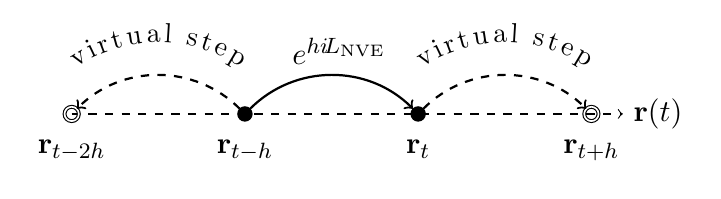
\begin{tikzpicture}
\draw[->, dashed]   (0,0.0) -- (7,0.0) node[right]{${\vt r}(t)$};
\node(0) at (0,0)[shape=circle,draw,double,scale=0.5]        {};
\node(1) at (2.2,0)[fill=black,shape=circle,draw,scale=0.5]        {};
\node(2) at (4.4,0)[fill=black,shape=circle,draw,scale=0.5]        {};
\node(3) at (6.6,0)[shape=circle,draw,double,scale=0.5] {};
\node(4) at (3.4,0.8)[] {$e^{\timestep \Liu{\tiny NVE}}$};
\node at (0.0,-0.2)[below]{${\vt r}_{t-2\timestep}$};
\node at (2.2,-0.2)[below]{${\vt r}_{t-\timestep}$};
\node at (4.4,-0.2)[below]{${\vt r}_{t}$};
\node at (6.6,-0.2)[below]{${\vt r}_{t+\timestep}$};
\path[->,thick] (1) edge [bend left=45] (2);
\path[dashed,->,thick,postaction={decorate,decoration={raise=2.5ex,text along path,text align=center,text={|\small|virtual step}}}] (0) to [bend left=45] (1);
\path[dashed,->,thick] (1) edge [bend right=45] (0);
\path[dashed,->,thick,postaction={decorate,decoration={raise=2.5ex,text along path,text align=center,text={|\small|virtual step}}}] (2) to [bend left=45] (3);
\path[dashed,->,thick] (2) edge [bend left=45] (3);
\end{tikzpicture}
\caption{Schematic representation}
\label{fig:virtual steps}
\end{figure}

In addition, $\refined K$ must be reevaluated after the action of propagator $e^{\frac{\timestep}{2n} {\mathcal L}_0}$, which scales both $\vt p$ and $\vt \pi$ by a factor $e^{-\alpha_1^\ast \frac{\timestep}{2n}}$.
Because such action leaves the positions and quaternions intact and, as a consequence, the matrix $\refined{\mathbf \Omega}(\vt r, \vt q, \timestep^2)$ in Eq.~\eqref{eq:modified kinetic energy} remains unaltered, the reevaluation of $\refined K$ is done as simply as ${\refined K} = e^{-\alpha_1^\ast \frac{\timestep}{n}} {\refined K}^\ast$.

Finally, we recall that configurations are sampled from a distribution proportional to $e^{-\beta \refined{\Ham{}}}$.
Notwithstanding, it is possible to compute ensemble averages consistent with a distribution proportional to $e^{-\beta \Ham{}}$, which would have been obtained if $\timestep \to 0$.
For this, we simply need to reweight any computed observable $A$ in accordance with \cite{Torrie_1977}
\begin{equation}
\label{eq:reweighting}
%\langle A \rangle_0 = \frac{\sum\limits_{i=1}^{N_s} A(\vt x_i) \exp \left[{\frac{\refined{\Ham{}}(\vt x_i) - {\Ham{}}(\vt x_i)}{k_\text{\tiny B} T}}\right]}{\sum\limits_{i=1}^{N_s} \exp \left[{\frac{\refined{\Ham{}}(\vt x_i) - {\Ham{}}(\vt x_i)}{k_\text{\tiny B} T}}\right] },
\langle A \rangle_0 = \frac{\left\langle A \exp \left({\frac{\refined{\Ham{}} - \Ham{}}{k_\text{\tiny B} T}}\right)\right\rangle_\timestep}{\left\langle \exp \left({\frac{\refined{\Ham{}} - \Ham{}}{k_\text{\tiny B} T}}\right)\right\rangle_\timestep}.
\end{equation}

A drawback of our approach is that the resulting integrator lacks time-reversal symmetry due to the asymmetric differentiation formulas.
As a matter of fact, long-term reversibility is not generally achievable with software that relies on floating-point arithmetics.
In any event, if short-term reversibility is a requirement, one can simply employ a symmetric five-point stencil formula, at the price of one additional force computation round per time step.
Higher-order derivative estimates can also be obtained in this fashion if necessary.

\section{Application to the Simulation of Liquid Water}
\label{sec:numerical_results}

In this section, we analyze the performance of our proposed NVT-MD method and compare its results to those obtained by employing both the method of \citeauthor{Kamberaj_2005} \cite{Kamberaj_2005} and the method of \citeauthor{Martyna_1996} \cite{Martyna_1996} with our described adaptations.

The system under study has periodic boundary conditions and contains 903 TIP3P \cite{Jorgensen_1983} water molecules at a density of 970~kg/m\textsuperscript{3}.
The 12-6 Lennard-Jones and damped Coulombic interactions were truncated at 10 \AA and smoothed by a switching function over the range from 9.5 \AA to 10 \AA, such as done in Ref.~\citenum{Silveira_2017}. 
The damping of Coulombic interactions was done by a factor $\text{erfc}(-\alpha r)$, with $\alpha = 0.29~\text{\AA}^{-1}$.
In addition, all thermostated simulations were carried out considering a time-scale constant $t_d = 100~\text{fs}$.

We start by examining the departure of the \textit{refined} Hamiltonian from the specified one in NVE simulations.
This is the most direct way of determining the importance of the discretization errors \cite{Engle_2005}, which is essential for discussing the NVT case.
In Fig.~\ref{fig:nve} we show the time evolution of both $\refined{\Ham{}}$ (dotted lines) and $\Ham{}$ (solid lines) for the water system using different time-step sizes ($\timestep$).
For this, we used the numerical scheme of Eq.~\eqref{eq:splitting NVE} with the unsplit solution of Ref.~\citenum{Silveira_2017} applied for the rotations.
The four-point differentiation formulas presented in Sec.~\ref{sec:refined_method} were employed for computing the refined kinetic energy.
As expected, $\refined{\Ham{}}$ is very well conserved and close to $\Ham{}$ for $\timestep = 1~\text{fs}$, but rapidly departs from $\Ham{}$ when $\timestep$ increases.
It is worth remarking that $\refined{\Ham{}}$ corresponds to a simple and, most importantly, computationally inexpensive approximation of the truly conserved shadow Hamiltonian.
As a result, we observe increasing fluctuations in $\refined{\Ham{}}$ for $\timestep = 3~\text{fs}$ and $\timestep = 4~\text{fs}$.
This is an indication that
1) the employed four-point formulas do not provide derivatives with the required accuracy or
2) the high-order terms of the Baker-Campbell-Hausdorff series (see Appendix \ref{sec:rigid body shadow hamiltonian}) would have a non-negligible contribution to the shadow Hamiltonian.

\begin{figure}
	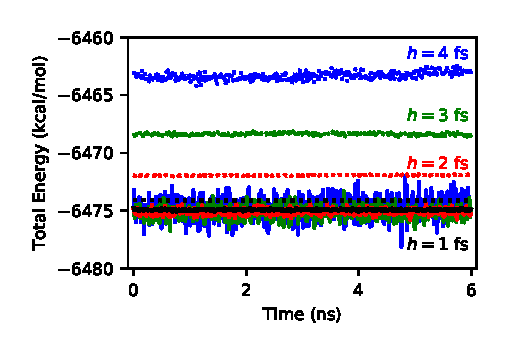
\includegraphics{Figures/NVE.eps}
	\caption{Specified Hamiltonian $\Ham{}$ (solid lines) and refined Hamiltonian $\refined{\Ham{}}$ (dotted lines) for different time-step sizes ($\timestep$) obtained from NVE MD simulations of 903 TIP3P \cite{Jorgensen_1983} water molecules using the numerical scheme of Eq.~\eqref{eq:splitting NVE} with the unsplit rotation method \cite{Silveira_2017}.}
	\label{fig:nve}
\end{figure}

 \subsection*{Numerical Stability}

The explicit inclusion of the \textit{refined} Hamiltonian in a computationally cheap NVT integrator is achieved at the cost of losing the time-reversibility.
This poses the question whether the symmetry loss will influence the long-term stability.

Here we define the energy drift, denoted by $R$, as the the rate of change of energy with time, which corresponds to the angular coefficient obtained from linear regression fitting.
Recall that the quantity expected to be conserved along the simulation is $\widetilde{H}$ (Eq.~\ref{eq:this extended energy}) for our method, which from now on will be referred as ``This work''.
On the other hand, the symmetric scheme due to \citeauthor{Martyna_1996} \cite{Martyna_1996} should preserve $H$ (Eq.~\ref{eq:nvt extended energy}).
In Fig.~\ref{fig:energy_drift}, we present the computed $R$ as a function of the time-step size, and one can see that for these numerical schemes the energy starts to drift upwards from $\timestep$ = 5 fs. 
Also, the long-term stability is only modestly improved by our method. Evidently, the impact of the lack of symmetry on $R$, if any, is negligible.
Fig.~\ref{fig:energy_drift} also contains the drift in $\refined{\Ham{}}$ for the NVE method \cite{Silveira_2017} (circles), which almost coincides with the results of our method. It is worth mentioning that the stability threshold for the NVE method corresponds to $\timestep$ = 6 fs.
The NVT methods discussed so far allow to extend that limit to 10 fs (see Table~\ref{table:stability} in the Supplementary Material). As one can notice in Fig.~\ref{fig:energy_drift}, the drift in the \textit{refined} Hamiltonian part for our NVT method (squares) remains bounded for all the time-step sizes considered, so the thermostat is stabilizing the numerical integration.
This has already been noticed by Davidchack\cite{Davidchack_2009}, and previously by Bond \textit{et al.} \cite{Bond_2007}, who in this respect stated that ``the thermostat acts as a sort of reservoir for numerical error''.

\begin{figure}
	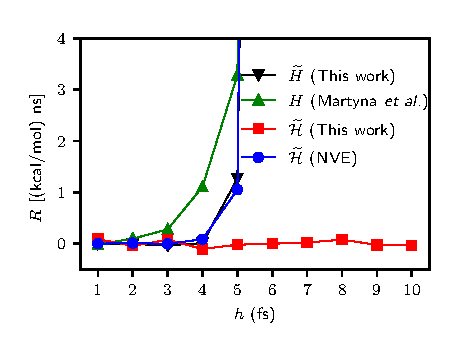
\includegraphics{Figures/energy_drift.eps}
    \caption{Influence of the time-step size ($\timestep$) on the long-time drift ($R$) in: the extended energy ($\refined{H}$, down triangles) and its \textit{refined} Hamiltonian ($\refined{\Ham{}}$, squares) part for our NVT method, as well as in the extended energy ($H$, up triangles) for the method due to \citeauthor{Martyna_1996} \cite{Martyna_1996} and in the \textit{refined} Hamiltonian ($\refined{\Ham{}}$, circles) for the numerical scheme of Eq.~\ref{eq:splitting NVE} with unsplit solution of rotation.}
	\label{fig:energy_drift}
\end{figure}

To end this section, we present in Fig.~\ref{fig:num_stab} the anomalous behavior encountered when using the method of \citeauthor{Kamberaj_2005} \cite{Kamberaj_2005}.
Particularly, one can see from Fig.~\ref{fig:num_stab} (a) that for each time-step size the extended energy drifts upwards until reaching a point at which the integrator becomes stable.
It should be remarked that these results were double-checked by using the LAMMPS software package \cite{Plimpton_1995}. 
As already mentioned, the scheme due to \citeauthor{Kamberaj_2005} \cite{Kamberaj_2005} couples separate chains of Nos\'{e}-Hoover thermostats on the rotational and translational degrees of freedom.
Considering a factorization scheme different to the one employed by those authors, Davidchack \cite{Davidchack_2009} discovered the existence of energy flows between the two thermostats.
To the best of our knowledge, this finding did not result in a revision in the literature of the method of \citeauthor{Kamberaj_2005} \cite{Kamberaj_2005}.
As can be seen in Fig.~\ref{fig:num_stab} (b), where we depict the energy of each thermostat, that flux is also observed for the scheme due to \citeauthor{Kamberaj_2005} \cite{Kamberaj_2005}.
In addition, the negative values of energy correspond to the thermostat coupled to the translational degrees of freedom, so the energy is flowing from this thermostat to the one coupled to the rotational degrees of freedom.
Interestingly, Fig.~\ref{fig:num_stab} (b) suggests that a unique steady state is established, and the time to reach the steady state decreases with $\timestep$. As far as we know, this behavior has not been reported before.

\begin{figure}
	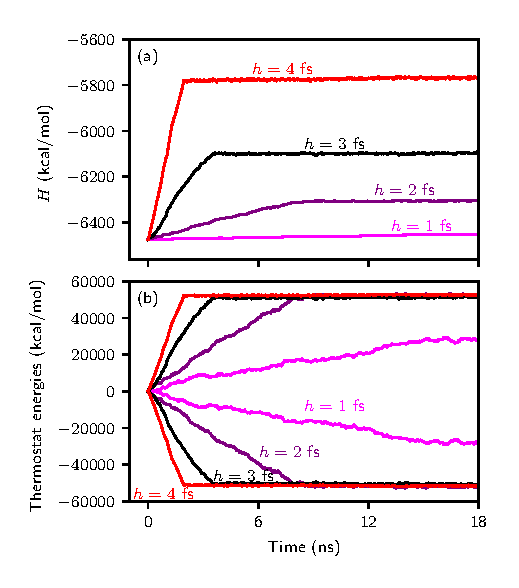
\includegraphics{Figures/numerical_stability.eps}
    \caption{Long-time drift in (a) the extended energy and (b) in each thermostat energy for the NVT method introduced by \citeauthor{Kamberaj_2005} \cite{Kamberaj_2005}. In part (b), the negative values correspond to the thermostat coupled to the translational degrees of freedom, so the energy is flowing to the thermostat coupled to the rotational degrees of freedom.}
	\label{fig:num_stab}
\end{figure}

\subsection*{Effect of Discretization Errors on Equilibrium Thermodynamic Properties}

In the previous section we showed that the energy drift is mainly localized within the thermostat variables.
It is then reasonable to ask if this leads to a more ``accurate'' sampling of the physical system.
To answer this question, we turn our attention to the discretization errors.

In Fig.~\ref{fig:properties} we show the computed average of some thermodynamic properties as a function of $\timestep$. The simulations were carried out specifying T = 298 K and the analyzed quantities correspond to temperature ($T$), potential energy ($U$) and virial ($W$) per molecule, as well as the constant-volume heat capacity ($C_v$).
The lines are a guide for the eye. 
Also, the horizontal dotted lines (black) help to visualize the departure of the computed averages with increasing $\timestep$.
They correspond to the results obtained employing $\timestep$ = 1 fs for the numerical scheme proposed in this paper.
We have included the results of applying our method but using the approximate solution of rotation due to Miller \textit{et al.} \cite{Miller_2002}, which is denoted as ``This work (NO-SQUISH)''.
The temperature values of Fig.~\ref{fig:properties} (a) were computed from the simulated kinetic energies assuming equipartition, ie $2 \langle K \rangle = (6N -3) k_b T$.

Despite the non-equilibrium process ocurring within the thermostats, it is worth showing the results obtained with the method of \citeauthor{Kamberaj_2005} \cite{Kamberaj_2005}, because that is not the only problematic issue.
Particularly, from Fig.~\ref{fig:properties} (a) we note that the simulated temperature decreases systematically with $\timestep$.
This behavior is observed in NVE simulations\cite{Davidchack_2009,Silveira_2017}, reflecting that the kinetic energy is weakly controlled in that factorization scheme.
As a result, the potential energy and virial are not severely influenced by $\timestep$ as they are in the scheme of \citeauthor{Martyna_1996} \cite{Martyna_1996}. Figs.~\ref{fig:properties} (a)-(b) clearly show that the temperature control described in Sec.~\ref{sec:nvt} leads to a severely degraded accuracy in $\langle U \rangle$, which systematically increases with $\timestep$.
As demonstrated in Fig.~\ref{fig:nve}, the discretization errors are non-negligible even for a small step size of 2 fs.
Thus, the results for the method of \citeauthor{Martyna_1996} \cite{Martyna_1996} can be interpreted as follows: if the kinetic energy is restricted to adopt a certain value, in accordance with the target temperature, the unavoidable discretization errors will accumulate in the remaining degrees of freedom.

From Fig.~\ref{fig:properties} it becomes clear that our method yields significantly improved results: we are able to simultaneously reproduce the specified temperature and the other thermodynamic properties. 
This is true also for the results corresponding to the use of the NO-SQUISH method\cite{Miller_2002} in the NVE part of the integrator.
Mathematically, the derivation of the refined Hamiltonian was facilitated by the fewer number of operators associated with the unsplit solution of rotation.
However, the accuracy of the approximate solution is very high for the time step sizes considered\cite{Silveira_2017} and this explains the good agreement.
Also note that a small, still clearly influencing systematic error is present in our scheme, as both temperature and potential energy are slightly modified by $\timestep$. This could, in principle, be remediated by using a higher-order approximation to the shadow Hamiltonian. 

With the aim of highlighting the importance of reweighting, in Fig.~\ref{fig:free_energy} we show for each time-step size the free energy difference per water molecule ($\Delta F/N$, circles) between the sampled and target states.
$\Delta F$ corresponds to the logarithm of the averaged denominator of Eq.~\ref{eq:reweighting}.
As expected, the free energy is only negligible for $h$ = 1 fs.

In Fig.~\ref{fig:free_energy} we also depict the \textit{refined} temperature ($\refined{T}$, squares), calculated by means of the generalized equipartition theorem, given by Eq.~\ref{eq:equipartition}.
Of course, as $\refined{T}$ is indirectly controlled by means of Eq.~\ref{eq:thermostat_force}, it is expected to reproduce the target temperature.
Indeed, for all the time-step sizes considered the agreement is excellent.

\begin{figure}
	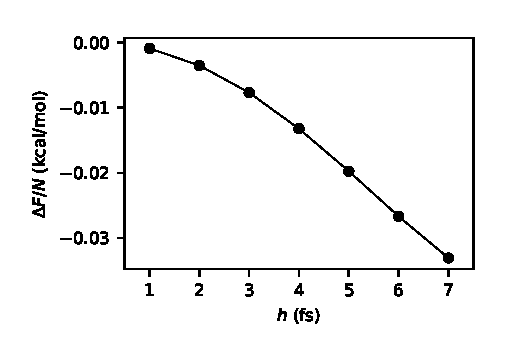
\includegraphics{Figures/Free_Energy.eps}
	\caption{Free Energy}
	\label{fig:free_energy}
\end{figure}

We end this section with a discussion of the effect of discretization errors on the kinetic energy partition.
In Fig.~\ref{fig:energy_partition} we show the translational ($K_t$) and rotational ($K_r$) kinetic energies as a function of the time-step size, and compare the results with the expected values assuming equipartition, which are calculated from the kinetic energy $\langle K \rangle$, as follows: $\langle K_t \rangle_{eq}$ = $(\langle K \rangle /(6N -3)) \times (3N - 3)$ and $\langle K_r \rangle_{eq}$ = $(\langle K \rangle /(6N -3)) \times 3N$.

In our previous work\cite{Silveira_2017}, we demonstrated that in the NVE case the rotational kinetic energy is more influenced by the time-step size because the rotational degrees of freedom are the fastest modes in the rigid model of water. 
We see that the method of \citeauthor{Kamberaj_2005} \cite{Kamberaj_2005} reproduces the behavior of the NVE case, as noted before.
The results of Fig.~\ref{fig:energy_partition} (b), which were obtained for the numerical scheme of \citeauthor{Martyna_1996} \cite{Martyna_1996}, are similar to Fig.~\ref{fig:energy_partition} (c), in the sense that the simulated translational and rotational kinetic energies deviate almost symmetrically and in opposite directions. Also, they do so contrary to what is expected: the translational kinetic energy should be smaller than the rotational one.
From Fig.~\ref{fig:energy_partition} it is clear that our method corrects that serious disruption for time-step sizes up to 5 fs.


\begin{figure*}
	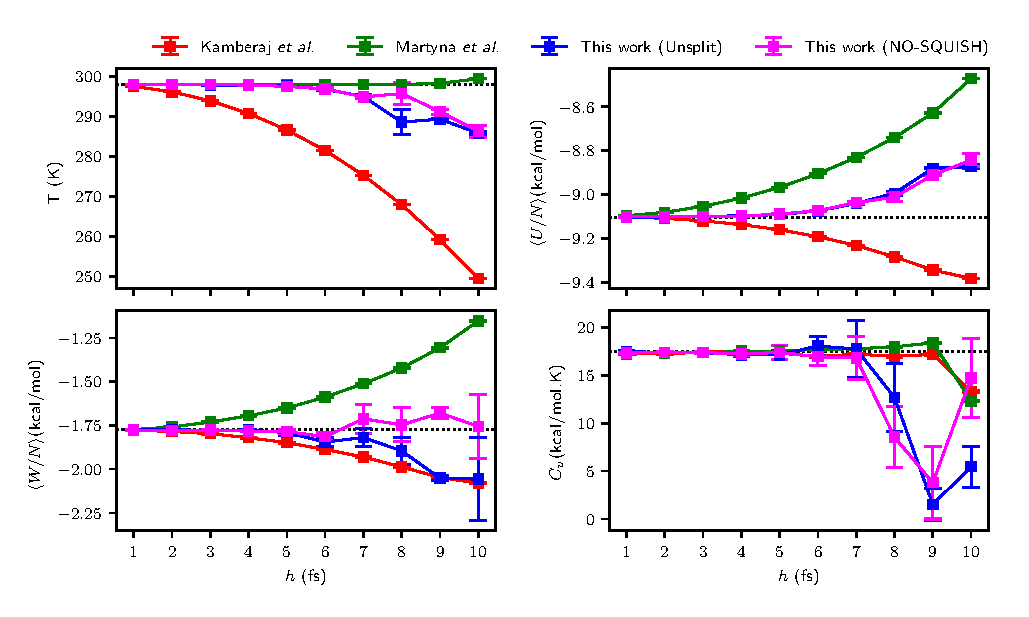
\includegraphics{Figures/thermodynamic_properties.eps}
	\caption{Effect of the time-step size on the thermodynamic properties and of 903 TIP3P\cite{Jorgensen_1983} water molecules in NVT MD simulations employing...}
	\label{fig:properties}
\end{figure*}

\begin{figure*}
	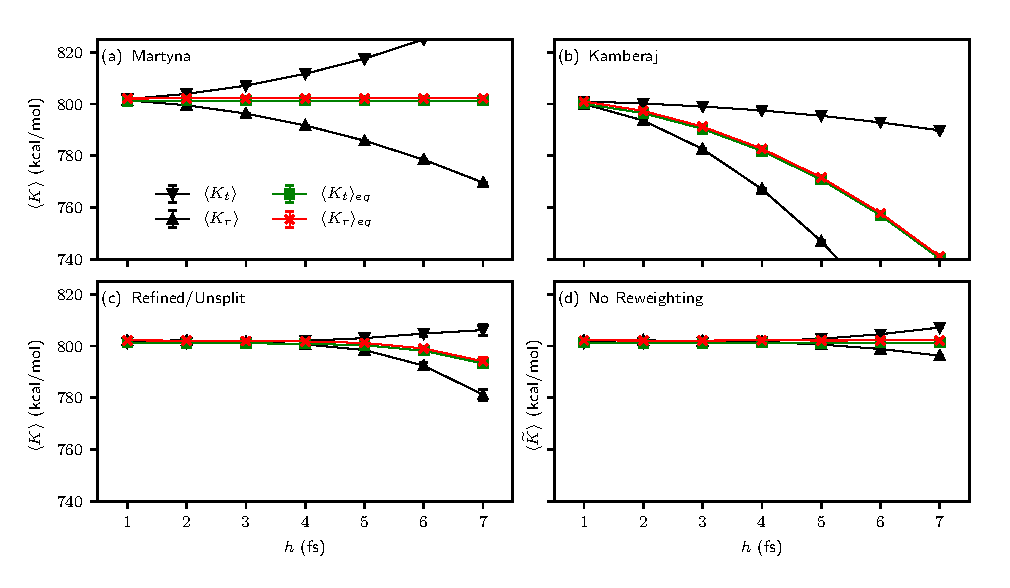
\includegraphics{Figures/energy_partition.eps}
		\caption{Effect of the time-step size on ... 903 TIP3P\cite{Jorgensen_1983} water molecules in NVT MD simulations employing...}
	\label{fig:energy_partition}
\end{figure*}


\section{Concluding Remarks}
\label{sec:conclusion}

\begin{acknowledgement}
	The authors acknowledge the financial support provided by Petrobras (project code CENPES 16113).
\end{acknowledgement}

\appendix
\numberwithin{equation}{section}

\section{Shadow Hamiltonian Approximation for Rigid Bodies}
\label{sec:rigid body shadow hamiltonian}

For two non-commutative Liouville operators $\Liu A$ and $\Liu B$ and a real constant $\timestep$, the symmetric Baker-Campbell-Hausdorff (BCH) formula can be expressed as \cite{Hairer_2006}
\begin{equation}
\label{eq:symmetric BCH}
\begin{split}
&e^{\frac{\timestep}{2} \Liu B} e^{\timestep \Liu A} e^{\frac{\timestep}{2} \Liu B} = \\
&= e^{\timestep (\Liu A + \Liu B) + \frac{\timestep^3}{24} \left[2 \Liu A + \Liu B,[\Liu A,\Liu B]\right] + \mathcal{O}(\timestep^5)},
\end{split}
\end{equation}
where $[X,Y]$ is the commutator of operators $X$ and $Y$, defined as $[X,Y] = XY - YX$.
The remaining terms of the infinite series involve ever-deepening, nested commutators \cite{Hairer_2006}.

Let us now represent the operators $\Liu A$ and $\Liu B$ using Poisson brackets involving Hamiltonians $\Ham A$ and $\Ham B$, that is, $\Liu A = \{\circ,\Ham A\}$ and $\Liu B = \{\circ,\Ham B\}$.
By employing the properties of anti-commutativity and Jacobi identity \cite{Hairer_2006}, we can deduce that
\begin{align*}
[\Liu A,\Liu B] &= \{\{\circ,\Ham B\},\Ham A\} - \{\{\circ,\Ham A\},\Ham B\} = \\
&= -\{\Ham A,\{\circ,\Ham B\}\} - \{\Ham B,\{\Ham A,\circ\}\} = \\
&= \{\circ,\{\Ham B,\Ham A\}\} = \\
&= \{\circ,{\Liu A} {\Ham B}\}.
\end{align*}

This means that the commutator $[\Liu A,\Liu B]$ is, in fact, a new Liouville operator $\Liu C$ whose associated Hamiltonian is $\Ham C = {\Liu A}{\Ham B}$.
By applying this procedure recursively, we can rewrite the right-hand side of Eq.~\eqref{eq:symmetric BCH} as $e^{\timestep \Liu S}$, where $\Liu S$ is the Liouville operator whose associated Hamiltonian is
\begin{equation*}
\label{eq:general shadow hamiltonian}
\refined{\Ham{}} = \Ham A + \Ham B + \frac{\timestep^2}{24} (2 \Liu A + \Liu B){\Liu A}{\Ham B} + \mathcal{O}(\timestep^4).
\end{equation*}

Therefore, a splitting method meant to approximately reproduce the dynamics of a system with Hamiltonian $\Ham{} = \Ham A + \Ham B$ will, in fact, reproduce exactly (putting round-off issues aside) the dynamics of another system with Hamiltonian $\refined{\Ham{}}$ as above.
In the literature, $\refined{\Ham{}}$ is usually referred to as a shadow Hamiltonian.

In the development that follows, we consider a single rigid body and, in the end, we generalize the result for a system of rigid bodies.

For the splitting introduced in Section~\ref{sec:nve}, $\Ham A = K(\vt p, \vt q, \vt \pi)$ and $\Ham B = U(\vt r, \vt q)$ with the corresponding Liouviller operators $\Liu{A} = \tr{K_{\vt p}}\diff{}{\vt r} + \tr{K_{\vt \pi}}\diff{}{\vt q} - \tr{K_{\vt q}}\diff{}{\vt \pi}$ and $\Liu{B} = -\tr{U_{\vt r}}\diff{}{\vt p} - \tr{U_{\vt q}}\diff{}{\vt \pi}$, with $K_{x}$ and $U_{x}$ being the gradient of the kinetic and potential energies, respectively.
We first obtain $\Liu A \Ham B = \tr{K_{\vt p}} U_{\vt r} + \tr{K_{\vt \pi}} U_{\vt q}$, and we find that
\begin{align*}
\Liu A \Liu A \Ham B &= \tr{K_{\vt p}} U_{\vt r \vt r} K_{\vt p}
+ 2 \tr{K_{\vt \pi}} U_{\vt r \vt q} K_{\vt p}
+ \tr{K_{\vt \pi}} U_{\vt q \vt q} K_{\vt \pi} \\
&+ \tr{K_{\vt \pi}} K_{\vt \pi \vt q} U_{\vt q}
- \tr{K_{\vt q}} K_{\vt \pi \vt \pi} U_{\vt q},
\end{align*}
where the fact that $\tr{U_{\vt q \vt r}} = U_{\vt r \vt q}$ has been exploited.
As reported in Ref.~\citenum{Silveira_2017}, the identity $\tr{\mt B}(\vt q) {\vt \pi} = -\tr{\mt B}(\vt \pi) {\vt q}$ is useful for performing differentiations.
The first-order derivatives of $K$ with respect to $\vt p$, $\vt q$, and $\vt \pi$ are, respectively,
\begin{align*}
&K_{\vt p} = {\mt M}^{-1} {\vt p}, \\
&K_{\vt q} = -\frac{1}{2} {\mt B}(\vt \pi) {\vt \omega}, \; \text{and} \\
&K_{\vt \pi} = \frac{1}{2} {\mt B}(\vt q) {\vt \omega},
\end{align*}
where $\vt \omega = \frac{1}{2} {\mt I}^{-1} \tr{\mt B}(\vt q) \vt \pi = -\frac{1}{2} {\mt I}^{-1} \tr{\mt B}(\vt \pi) \vt q$.\cite{Silveira_2017} Hence,
\begin{gather*}
\tr{K_{\vt p}} U_{\vt r \vt r} K_{\vt p} = \tr{\vt p} {\mt M}^{-1} U_{\vt r \vt r} {\mt M}^{-1} {\vt p}, \\
\tr{K_{\vt \pi}} U_{\vt r \vt q} K_{\vt p} = \frac{1}{2} \tr{\vt \omega} \tr{\mt B}(\vt q) U_{\vt r \vt q} {\mt M}^{-1} {\vt p}, \\
\tr{K_{\vt \pi}} U_{\vt q \vt q} K_{\vt \pi} = \frac{1}{4} \tr{\vt \omega} \tr{\mt B}(\vt q) U_{\vt q \vt q} {\mt B}(\vt q) \vt \omega.
\end{gather*}

As $\diff{\tr{\vt \omega}}{\vt \pi} = \frac{1}{2} {\mt B}(\vt q) {\mt I}^{-1}$, the second-order derivative of $K$ with respect to $\vt \pi$ turns out to be
\begin{equation*}
K_{\vt \pi \vt \pi} = \frac{1}{4} {\mt B}(\vt q) {\mt I}^{-1} \tr{\mt B}(\vt q).
\end{equation*}

Pre-multiplication by $\tr{K_{\vt q}}$ will introduce a product $\tr{\mt B}(\vt \pi) {\mt B}(\vt q)$, which has been shown in Ref.~\citenum{Silveira_2017} to be equal to ${\mt S}\left( \tr{\mt B}(\vt \pi) {\vt q} \right) = -2 {\mt S}({\mt I} {\vt \omega})$, where the operator ${\mt S}(\cdot)$ builds a skew-symmetric matrix from the entries of a vector.
In addition, post-multiplication by $U_{\vt q}$ will introduce a product $\tr{\mt B}(\vt q) U_{\vt q}$, which is equal to $-2 {\vt \tau}^b$, where ${\vt \tau}^b$ is the body-fixed frame representation of the torque.
Then, the fact that ${\mt S}(\vt x) {\vt y} = -{\mt S}(\vt y) {\vt x}$ leads to
\begin{equation*}
\tr{K_{\vt q}} K_{\vt \pi \vt \pi} U_{\vt q} = \frac{1}{2} \tr{\vt \omega} {\mt S}({\mt I}^{-1} {\vt \tau}^b) {\mt I} {\vt \omega} = 0,
\end{equation*}
which is a null term as it corresponds to the quadratic form of a skew-symmetric matrix.
Another helpful identity taken from Appendix B of Ref.~\citenum{Silveira_2017} is ${\mt B}(\vt q){\vt \omega} = ( \sum_{k=1}^3 \omega_k \hat{\mt B}_k ) \vt q$, where each $\hat{\mt B}_k$ is a skew-symmetric permutation matrix (i.e.
$\tr{\hat{\mt B}}_k = -\hat{\mt B}_k$).
This allows us to obtain
\begin{align*}
K_{\vt \pi \vt q} &= \frac{1}{2} (\diff{\tr{\vt \omega}}{\vt q}) \tr{\mt B}(\vt q) + \frac{1}{2} \sum_{k=1}^3 \omega_k \tr{\hat{\mt B}}_k = \\
&= -\frac{1}{4} {\mt B}(\vt \pi) {\mt I}^{-1} \tr{\mt B}(\vt q) - \frac{1}{2} \sum_{k=1}^3 \omega_k \hat{\mt B}_k.
\end{align*}

Pre-multiplication by $\tr{K_{\vt \pi}}$ and post-multiplying $U_{\vt q}$, followed by some algebraic transformations, ultimately lead to
\begin{equation*}
\tr{K_{\vt \pi}} K_{\vt \pi \vt q} U_{\vt q} = -\frac{1}{2} \tr{\vt \omega} \tr{\mt S}({\mt I}^{-1} {\vt \tau}^b) {\mt I} {\vt \omega} + \frac{1}{2} \tr{\vt \omega} {\mt S}({\vt \tau}^b){\vt \omega}.
\end{equation*}
Both terms in the right-hand side of the equation above are identically null. 
Now, we are able to evaluate $\Liu A \Liu A \Ham B $, which is
\begin{align*}
\Liu A \Liu A \Ham B = &\tr{\vt p} {\mt M}^{-1} U_{\vt r \vt r} {\mt M}^{-1} {\vt p} + \tr{\vt \omega} \tr{\mt B}(\vt q) U_{\vt r \vt q} {\mt M}^{-1} {\vt p}
+ \\
&\frac{1}{4} \tr{\vt \omega} \tr{\mt B}(\vt q) U_{\vt q \vt q} {\mt B}(\vt q) \vt \omega.
\end{align*}
The remaining term to obtain $H_s$ is simply given by 
\begin{align*}
\Liu B \Liu A \Ham B &= -\tr{U_{\vt r}} \tr{K_{\vt p \vt p}} U_{\vt r} - \tr{U_{\vt q}} \tr{K_{\vt \pi \vt \pi}} U_{\vt q} = \\
&= -\tr{\vt F} {\mt M}^{-1} {\vt F} - \tr{\vt \tau}_b {\mt I}^{-1} {\vt \tau}_b.
\end{align*}

As will become clear below, it is convenient to rewrite the total kinetic energy of the original system, Eq.~\eqref{eq:kinetic energy}, as a quadratic form
\begin{equation*}
K = \frac{1}{2} \tr{ \left[\begin{array}{c} \vt p \\ \vt \pi \end{array}\right]} {\mt \Omega}(\vt q) \left[\begin{array}{c} \vt p \\ \vt \pi \end{array}\right],
\end{equation*}
where $\mt \Omega$ is a symmetric, block-diagonal matrix of size $7N \times 7N$ defined as
\begin{equation}
\label{eq:block-diagonal inverse mass tensor}
{\mt \Omega} = \left[\begin{array}{cc}
{\mt M}^{-1} & \mt 0 \\
\mt 0 & \frac{1}{4} {\mt B}(\vt q) {\mt I}^{-1} \tr{\mt B}(\vt q)
\end{array}\right].
\end{equation}

We now proceed to show the final expression of $H_s$, which results from grouping the terms corresponding to forces and torques in the \textit{modified} potential energy $\tilde{U}$, given by
\begin{equation*}
\refined U = U - \frac{\timestep^2}{24} \left( \tr{\vt F} {\mt M}^{-1} {\vt F} + \tr{\vt \tau} \tr{\mt A} {\mt I}^{-1} {\mt A} {\vt \tau} \right).
\end{equation*}
while the remaining terms can be recast in a compact matrix, as follows
\begin{equation*}
\refined K = \frac{1}{2} \tr{ \left[\begin{array}{c} \vt p \\ \vt \pi \end{array}\right]} \refined{\mathbf \Omega}(\vt r, \vt q) \left[\begin{array}{c} \vt p \\ \vt \pi \end{array}\right],
\end{equation*}
where
\begin{equation*}
\tilde{\mt \Omega} = {\mt \Omega} + \frac{\timestep^2}{6} \left( {\mt \Omega} {\mt U}_{\vt x \vt x} \tr{\mt \Omega} \right)
\end{equation*}
and
\begin{equation*}
{\mt U}_{\vt x \vt x} = \left[\begin{array}{cc}
U_{\vt r \vt r} & U_{\vt r \vt q} \\
U_{\vt q \vt r} & U_{\vt q \vt q}
\end{array}\right].
\end{equation*}

Finally, we have that
\begin{equation*}
\Ham S = \frac{1}{2} \tr{\left[\begin{array}{c} \vt p \\ \vt \pi \end{array}\right]} \tilde{\mt \Omega} \left[\begin{array}{c} \vt p \\ \vt \pi \end{array}\right] + \tilde{U} + \mathcal{O}({\timestep}^4),
\end{equation*}

Although $\refined{\mathbf \Omega}$ is still symmetric, it is no longer a block-diagonal matrix like $\mt \Omega$, due to the inter-body interactions accounted for in $U(\vt r, \vt q)$ and to the dependency of forces and torques on both positions and orientations.
As a result, the modified kinetic energy cannot, in principle, be split into independent translational and rotational contributions.

\suppinfo

\bibliography{rigid_bodies}
\end{document}
